Không! Thông tin về các dòng điện và hiện điện thế giữa hai đầu mạch là chưa đủ để xác định giá trị của các điện trở (chúng ta có vô số nghiệm). Điều này nghe có vẻ bất ngờ, vì nếu biết điện trở thì chúng ta có thể xác định được dòng điện, nhưng điều ngược lại không phải lúc nào cũng khả thi. 

\ \ 

Sơ sài mà nói, nguyên nhân là bởi vì điện trở là các giá trị độc lập còn dòng điện là các giá trị liên hệ, dẫn tới rằng nếu biết điện trở thì ta có đủ phương trình để giải ra dòng điện, còn nếu biết dòng điện thì ta có ít phương trình độc lập hơn, tổng quát thì sẽ không đủ để giải ra điện trở. 

\begin{center}
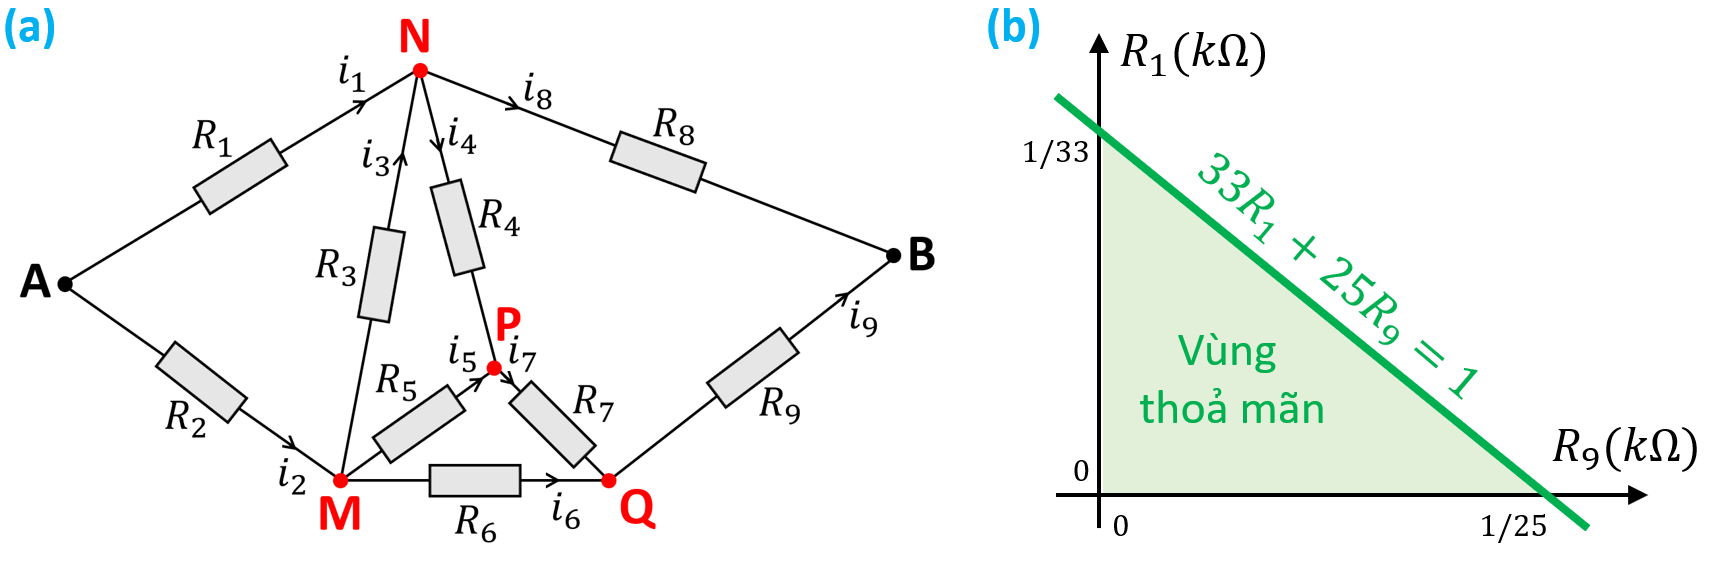
\includegraphics[width=\textwidth,keepaspectratio]{Problem_2/Figs/S2A.png}
\end{center}

\ \ 

Chi tiết hơn, cho mọi bộ giá trị điện thế $[\mathcal{V}(\text{M}),\mathcal{V}(\text{N}),\mathcal{V}(\text{P}),\mathcal{V}(\text{Q})]$ xác định tại các nút mạng M, N, P, Q (xem hình \textbf{a}) sao cho:
\begin{equation}
\mathcal{V}(\text{A}) > \mathcal{V}(\text{M}) > \mathcal{V}(\text{N}) > \mathcal{V}(\text{P}) > \mathcal{V}(\text{Q}) > \mathcal{V}(\text{B})   \ ,
\end{equation}
với mốc điện thế hai đầu A và B được chọn là $\mathcal{V}(\text{A})=1$, $\mathcal{V}(\text{B})=0$ (đơn vị $V$), thế thì dòng điện sẽ có chiều như mô tả (chảy từ nơi có điện thế cao xuống thấp) và bộ các giá trị điện trở (luôn luôn dương) là duy nhất:
\begin{equation}
\begin{split}
R_1 = \frac{\mathcal{V}(\text{A})-\mathcal{V}(\text{N})}{i_1} \ , \ R_9 = \frac{\mathcal{V}(\text{A})-\mathcal{V}(\text{M})}{i_2} \ , \ R_9 = \frac{\mathcal{V}(\text{M})-\mathcal{V}(\text{N})}{i_3} \ , & 
\\
R_4 = \frac{\mathcal{V}(\text{N})-\mathcal{V}(\text{P})}{i_4} \ , \ R_5 = \frac{\mathcal{V}(\text{M})-\mathcal{V}(\text{P})}{i_4} \ , \ R_6 = \frac{\mathcal{V}(\text{M})-\mathcal{V}(\text{Q})}{i_4} \ , &
\\
R_7 = \frac{\mathcal{V}(\text{P})-\mathcal{V}(\text{Q})}{i_4} \ , \ R_8 = \frac{\mathcal{V}(\text{N})-\mathcal{V}(\text{B})}{i_4} \ , \ R_9 = \frac{\mathcal{V}(\text{Q})-\mathcal{V}(\text{B})}{i_4} \ . 
\end{split}
\end{equation}
Mạch điện khi ấy thoả mãn tất cả các định luật Kirchhoff. Không thể xác định được chính xác và hữu hạn các giá trị khả dĩ $(R_1,R_9)$, do có vô số bộ điện thế $[\mathcal{V}(\text{M}),\mathcal{V}(\text{N}),\mathcal{V}(\text{P}),\mathcal{V}(\text{Q})]$ có thể chọn!

\ \ 

Mặc dù không thể xác định được chính xác $R_1$ và $R_9$, tuy nhiên chúng ta vẫn có thể xác định được vùng không gian giá trị điện trở khả dĩ $(R_1,R_9)$ có diện tích hữu hạn! Cụ thể hơn (xem hình \textbf{b}):
\begin{equation}
R_1 > 0 \ , \ R_2 > 0 \ \ , \ \ i_1 R_1 + i_2 R_2 < 1 \ .
\end{equation}
\begin{itemize}
    \item Chặn dưới $R_1 > 0$ và $R_2 > 0$: $\mathcal{V}(\text{M})$, $\mathcal{V}(\text{N})$ rất sát với $\mathcal{V}(\text{A})$ và $\mathcal{V}(\text{Q})$ rất sát với $\mathcal{V}(\text{B})$. Hai giới hạn này có thể được đồng thời thoả mãn, không có xung đột.
    \item Chặn trên $i_1 R_1 + i_2 R_2 < 1$: $\mathcal{V}(\text{N})$, $\mathcal{V}(\text{P})$,  $\mathcal{V}(\text{Q})$  rất sát với nhau.
\end{itemize}

\ \ 

\textit{Khi soạn các bài tập, do yếu tố con người nên chúng ta không thể tránh khỏi những vấn đề oái oăm, như không tồn tại đáp án hợp lý cho câu hỏi được nêu ra. Bài tập này được thiết kế để truyền tải thông điệp đó. Tất nhiên, câu hỏi của bài đã có gợi ý cho vấn đề của yêu cầu xác định điện trở, nhưng các bạn cần lưu ý rằng khi đề bài đã lỗi thì sẽ không tồn tại gợi ý như vậy đâu! Các bạn học sinh cần phải bình tĩnh, tự tin vào kiến thức của mình, và chứng minh rằng đáp án là vô nghiệm hoặc vô số nghiệm (nếu tìm được vùng giới hạn cho tập hợp các đáp án khả dĩ thì cũng rất tốt), hay thậm chí mạnh dạn chỉ thẳng ra điều chưa hợp lý của đề bài.}